\documentclass[tikz,border=2pt]{standalone}
\usepackage{amsmath}
\usetikzlibrary{arrows.meta,calc}
\begin{document}
% Harsanyi transformation of the contribution game: Nature draws (theta_1, theta_2) in {1/4, 2}^2,
% each profile w.p. 1/4. Player 1 sees only theta_1 (2 information sets of 2 nodes); player 2 sees
% only theta_2, not player 1's action (2 information sets of 4 nodes); 16 terminal nodes.
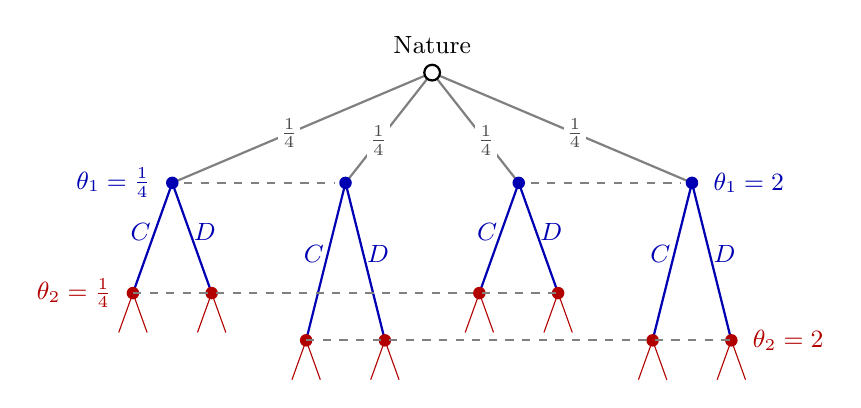
\begin{tikzpicture}[font=\small, >={Latex[length=2mm]},
    dec/.style={circle, fill, inner sep=1.6pt},
    nat/.style={circle, draw, thick, fill=white, inner sep=2pt}]
  % Nature's branches (order: (1/4,1/4), (1/4,2), (2,1/4), (2,2))
  \foreach \x in {-3.3,-1.1,1.1,3.3}
    \draw[thick, gray] (0,0) -- (\x,-1.4);
  \foreach \x/\p in {-3.3/0.55,-1.1/0.62,1.1/0.62,3.3/0.55}
    \node[gray!60!black, fill=white, inner sep=1pt] at ($(0,0)!\p!(\x,-1.4)$) {$\tfrac14$};
  % player 1's actions; player 2 nodes at y = -2.8 (theta_2 = 1/4) or -3.4 (theta_2 = 2)
  \foreach \x/\y in {-3.3/-2.8,-1.1/-3.4,1.1/-2.8,3.3/-3.4} {
    \draw[thick, blue!70!black] (\x,-1.4) -- node[left, pos=0.45, inner sep=1pt] {$C$} (\x-0.5,\y);
    \draw[thick, blue!70!black] (\x,-1.4) -- node[right, pos=0.45, inner sep=1pt] {$D$} (\x+0.5,\y);
    \foreach \dx in {-0.5,0.5} {
      \draw[red!70!black] (\x+\dx,\y) -- (\x+\dx-0.18,\y-0.5);
      \draw[red!70!black] (\x+\dx,\y) -- (\x+\dx+0.18,\y-0.5);
      \node[dec, red!70!black] at (\x+\dx,\y) {};
    }
    \node[dec, blue!70!black] at (\x,-1.4) {};
  }
  % player 1's information sets
  \draw[dashed, thick, gray] (-3.15,-1.4) -- (-1.25,-1.4);
  \draw[dashed, thick, gray] (1.25,-1.4) -- (3.15,-1.4);
  \node[blue!70!black, anchor=east] at (-3.45,-1.4) {$\theta_1=\tfrac14$};
  \node[blue!70!black, anchor=west] at (3.45,-1.4) {$\theta_1=2$};
  % player 2's information sets
  \draw[dashed, thick, gray] (-3.8,-2.8) -- (1.6,-2.8);
  \draw[dashed, thick, gray] (-1.6,-3.4) -- (3.8,-3.4);
  \node[red!70!black, anchor=east] at (-3.95,-2.8) {$\theta_2=\tfrac14$};
  \node[red!70!black, anchor=west] at (3.95,-3.4) {$\theta_2=2$};
  % Nature
  \node[nat, label={above:Nature}] at (0,0) {};
\end{tikzpicture}
\end{document}
